% Stewart Dulaney
% https://www.stewartdulaney.com
% This document was adapted from the templates posted at the following sources:
% https://www.cs.cmu.edu/~ckingsf/class/02-714/hw-template.tex
% http://www.math-cs.gordon.edu/courses/mat231/handouts/truth-table-latex.tex
%
\documentclass[11pt]{article}
\usepackage{amsmath,amssymb,amsthm,mathabx}
\usepackage{graphicx}
\usepackage[margin=1in]{geometry}
\usepackage{fancyhdr}
\usepackage{listings}
\lstset{
  basicstyle=\ttfamily,
  mathescape
}
\setlength{\parindent}{0pt}
\setlength{\parskip}{5pt plus 1pt}
\setlength{\headheight}{13.6pt}
\newcommand\question[2]{\vspace{.25in}\hrule\textbf{#1: #2}\vspace{.5em}\hrule\vspace{.10in}}
\renewcommand\part[1]{\vspace{.10in}\textbf{(#1)}}
\newcommand\answer{\vspace{.10in}\textbf{Answer: }}
\pagestyle{fancyplain}
\lhead{\textbf{\NAME\ (SID: \SID)}}
\chead{\textbf{HW\HWNUM}}
\rhead{CS 180, \today}
\begin{document}\raggedright
%Section A==============Change the values below to match your information==================
\newcommand\NAME{Stewart Dulaney}  % your name
\newcommand\SID{904-064-791}     % your ucla student id
\newcommand\HWNUM{5}              % the homework number
%Section B==============Put your answers to the questions below here=======================

\question{6.3}{}

\answer

\part{a}

\begin{figure}[h!]
  \centering
  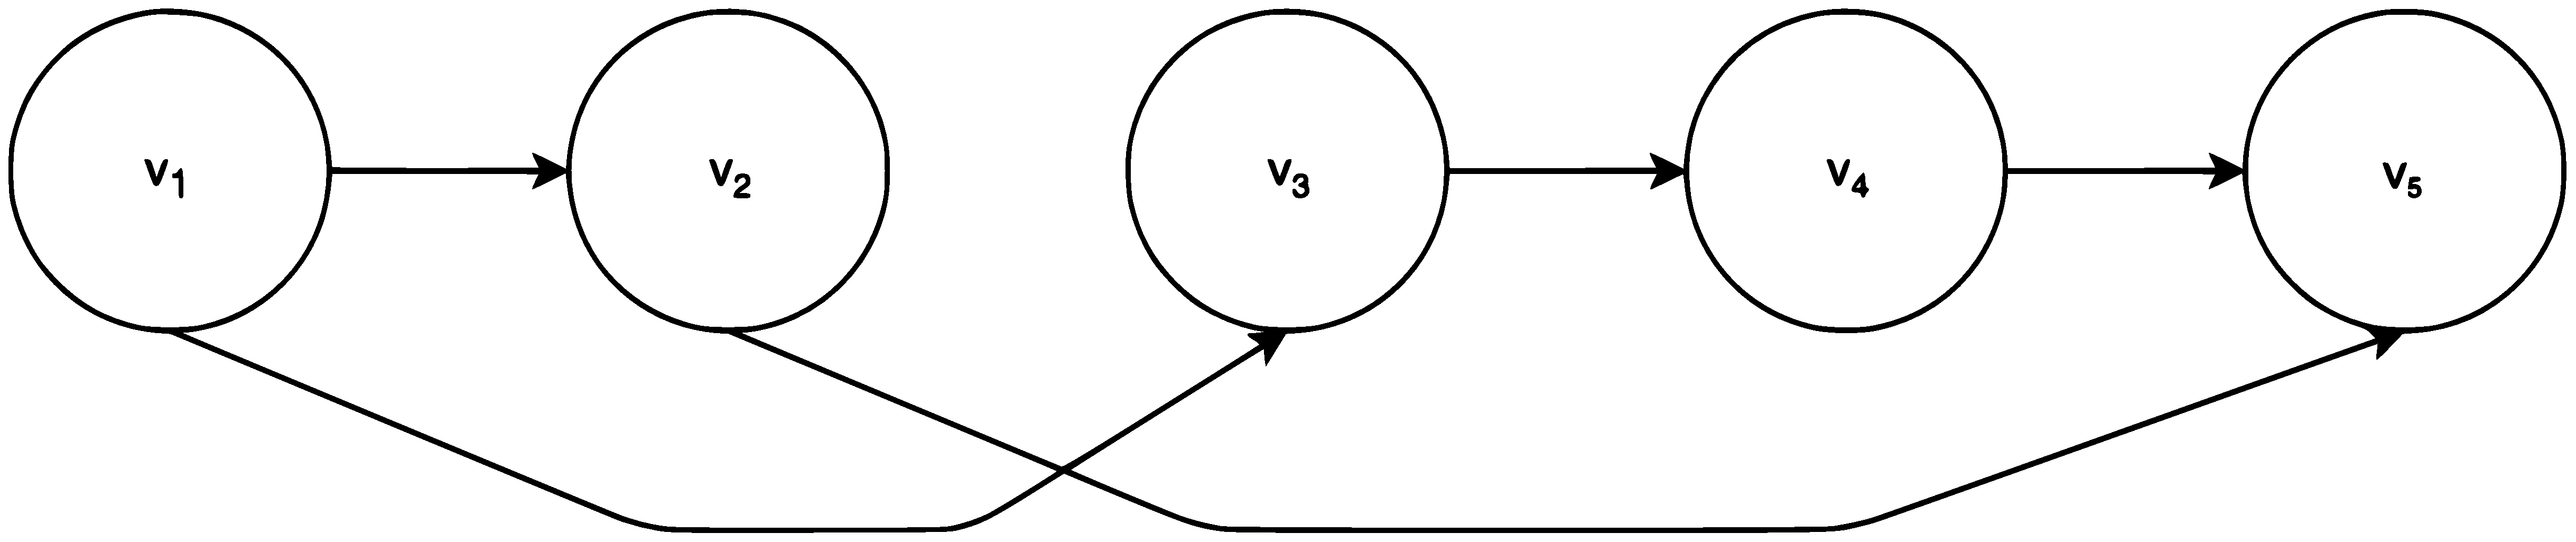
\includegraphics[width=\linewidth]{6.3a.eps}
  \caption{An ordered graph.}
  \label{fig:6.3a}
\end{figure}

The correct answer for this ordered graph is 3: The longest path from $v_1$ to $v_n$ uses the 3 edges $(v_1, v_3)$, $(v_3, v_4)$, and $(v_4, v_5)$. The given algorithm incorrectly returns the answer 2 for the path using the edges $(v_1, v_2)$ and $(v_2, v_5)$. 

\part{b}

We will use dynamic programming. We will use subproblems of the form $OPT[i] = $ length of the longest path from $v_1$ to $v_i$. Let $G = (V, E)$, $|V| = n$, and $|E| = m$. We use the value "$-\infty$" for $OPT[i]$ when there is not a path from $v_1$ to $v_i$. Base case: let $OPT[1] = 0$ because an ordered graph has no loops so the longest path from $v_1$ to $v_1$ is $0$.

This satisfies the three basic properties for a collection of subproblems:
\begin{enumerate}
  \item There are only a polynomial number of subproblems. \textbf{Namely, $n$.}
  \item The solution to the original problem can be easily computed from the solutions to the subproblems. \textbf{}
  \item There is a natural ordering on subproblems from “smallest” to “largest,” together with an easy-to-compute recurrence (as in (6.1) and (6.2)) that allows one to determine the solution to a subproblem from the solutions to some number of smaller subproblems. \textbf{We can iterate over subproblems from $2$ to $n$ in order of increasing vertex index. We can use the recurrence $OPT[i] = max_{(j, i) \in E}(OPT(j) + 1)$.}
\end{enumerate}

\clearpage

\begin{lstlisting}
Longest-Path-Ordered-Graph($V$, $E$)
  $n = |V|$
  Array $M[1...n]$
  $M[1] = 0$
  for $i = 2$,..., $n$
    $max = -\infty$
    for all edges $(j, i) \in E$
      if $M[j] \neq -\infty$
        if $max < M[j] + 1$
          $max = M[j] + 1$
    $M[i] = max$
  return M[n]
\end{lstlisting}

The outer for loop runs in $O(n)$. If we assume a simple directed graph (no multiple edges), there can be at most $(n - 1)$ edges $(j, i)$ for a given node $v_i$, and we can bound the inner for loop by $O(n)$. Therefore, the total time complexity is $O(n * n) = O(n^2)$.

\clearpage

\question{6.4}{}

\answer

\part{a}
Counterexample: let $n = 4$, $M = 10$, and the operating costs are given by the following table.

\begin{table}[h!]
\begin{tabular}{lcccc}
   & \multicolumn{1}{l}{Month 1} & \multicolumn{1}{l}{Month 2} & \multicolumn{1}{l}{Month 3} & \multicolumn{1}{l}{Month 4} \\
NY & 1                           & 3                           & 1                           & 2                           \\
SF & 2                           & 1                           & 2                           & 1                          
\end{tabular}
\end{table}

The correct answer is $[SF, SF, SF, SF]$ with $total\:cost = 2 + 1 + 2 + 1 = 6$. However, the given greedy algorithm incorrectly gives the plan $[NY, SF, NY, SF]$ with $total\:cost = 1 + 1 + 1 + 1 + 10 + 10 + 10 = 34$.

\part{b}

Let $n = 4$, $M = 1$, and the operating costs are given by the following table.

\begin{table}[h!]
\begin{tabular}{lcccc}
   & \multicolumn{1}{l}{Month 1} & \multicolumn{1}{l}{Month 2} & \multicolumn{1}{l}{Month 3} & \multicolumn{1}{l}{Month 4} \\
NY & 1                           & 10                           & 1                           & 10                           \\
SF & 10                           & 1                           & 10                           & 1                          
\end{tabular}
\end{table}

Brief explanation: the optimal plan $[NY, SF, NY, SF]$ has $total\:cost = 1 + 1 + 1 + 1 + 1 + 1 + 1 = 7$ and moves three times. Any other plan would have to pay an operating cost of at least $10$ in NY or SF, which would not be optimal.

\clearpage

\part{c}

We will use dynamic programming. We will use subproblems of the form $OPT_N(j)$, the minimum cost of a plan on months $1,...,j$ ending in NY, and $OPT_S(j)$, the minimum cost of a plan on months $1,...,j$ ending in SF. We can use the following two recurrences:\newline

$OPT_N(n) = N_n + min(OPT_N(n - 1), M + OPT_S(n - 1))$\\
$OPT_S(n) = S_n + min(OPT_S(n - 1), M + OPT_N(n - 1))$\newline

Our recurrences stem from the observation that the optimal plan either ends in NY or SF. If it ends in NY, it will incur a cost of $N_n$ plus the minimum of two quantities: (1) cost of the optimal plan on $n - 1$ months ending in NY, (2) cost of the optimal plan on $n - 1$ months ending in SF plus a moving cost of $M$. The same explanation holds if the optimal plan ends in SF.

Let $N = \{N_1,...,N_n\}$ and $S = \{S_1,...,S_n\}$.

\begin{lstlisting}
Minimum-Cost-Plan($n$, $M$, $N$, $S$)
  Array $MN[0...n]$
  Array $MS[0...n]$
  $MN[0] = 0$
  $MS[0] = 0$
  for $i = 1,...,n$
    $MN[i] = N_i + min(MN[i - 1], M + MS[i - 1])$
    $MS[i] = S_i + min(MS[i - 1], M + MN[i - 1])$
  if $MN[n] < MS[n]$
    return $MN[n]$
  else
    return $MS[n]$
\end{lstlisting}

The for loop runs for $n$ iterations and each iteration takes constant time. Therefore, the time complexity is $O(n * 1) = O(n)$. The space complexity is $O(2(n + 1)) = O(2n + 2) = O(n)$.

\clearpage

\question{6.6}{}

\answer

We will use dynamic programming with a similar strategy to that used in the Segmented Least Squares problem. We will use subproblems of the form $OPT[i]$, the value of the optimal solution on the set of words $W_i = \{w_1,...,w_i\}$. Let $S_{i, j}$ for $i \leq j$ be the slack of a line containing the words $w_i,...,w_j$ and $S_{i, j} = \infty$ if the total character count of these words exceeds the maximum line length $L$. Notice that in the optimal solution the last line ends with word $w_n$ and has to start with some word $w_j$. If we remove words $w_j,...,w_n$ we are left with a recursive subproblem on the words $w_1,...,w_{j - 1}$ that must be solved optimally. Therefore, we can use the following recurrence: $OPT[n] = min_{1 \leq j \leq n} (S_{i, n}^2 + OPT[j - 1])$ where the line of words $w_j,...,w_n$ is used in an optimum solution if and only if the minimum is obtained using index j (similar to the Segmented Least Squares problem).

Let $C = \{c_1,...,c_n\}$. The algorithm can be described as follows:

\begin{lstlisting}
Compute-Slacks($n$, $L$, $C$)
  Array $slacks[1...n][1...n]$
  for $i = 1,...,n$
    for $j = i,...,n$
      if $\sum_{x = i}^{j - 1} (c_x + 1) + c_j \leq L$
        slacks[i][j] = $L - \sum_{x = i}^{j - 1} (c_x + 1) + c_j$
      else
        $slacks[i][j] = \infty$
  return $slacks$

Compute-Optimum-Value($n$, $L$, $C$)
  Array $slacks[1...n][1...n]$ = Compute-Slacks($n$, $L$, $C$)
  Array $M[0...n]$
  $M[0] = 0$
  for $i = 1,...,n$
    $M[i] = min_{1 \leq j \leq i} (S_{j, i}^2 + M[j - 1])$
  return $M[n]$

Compute-Optimum-Solution($M$, $n$)
  Trace through array $M$ to recover the partition solution 
  corresponding to the optimal value $M[n]$
\end{lstlisting}

Compute-Slacks runs in $O(n^2)$ time because both for loops run for at most $n$ iterations. Compute-Optimum-Value has a term $O(n^2)$ for Compute-Slacks. It also has a for loop that runs for $n$ iterations, and each iteration takes $O(n)$. So in total Compute-Optimum-Value runs in $O(n^2 + n * n) = O(2n^2) = O(n^2)$. Compute-Optimum-Solution returns an optimal solution from the array of optimal values of the subproblems produced by Compute-Optimum-Value in $O(n)$ time.

\clearpage

\question{6.12}{}

\answer

We will use dynamic programming. We will use subproblems of the form $OPT(j)$, the minimum cost of a solution on servers $S_1,...,S_j$. The problem requires that we place a copy of the file at $S_j$ so that all searches will terminate there at the latest. We can use the recurrence $OPT(j) = c_j + min_{0 \leq i < j} (OPT(i) + {j - i \choose 2})$ with the base cases $OPT(0) = 0$ and ${1 \choose 2} = 0$. This is based on searching for which server to place the highest copy of the file before $S_j$. Assume the position $i$ server to be the desired location for the file in the optimal solution. We want to search over all $i$ to find the optimal solution. $OPT(i)$ is the cost for all servers up to $i$ by our assumption. The cost for the remaining servers $S_{i + 1},...,S_j$ is the sum of all access costs across that range, namely $0 + 1 + ... + (j - i - 1) = {j - i \choose 2}$. Lastly, we pay a $c_j$ placement cost for $S_j$. The array of optimal values of the subproblems can be built up in a loop with increasing $j$ that runs for $O(n)$ iterations, where each iteration takes $O(n)$ time. Therefore the algorithm to find the value $OPT(n)$ of the minimum total cost configuration runs in $O(n * n) = O(n^2)$ time. We can traverse the resulting array of optimum values of the subproblems in an additional $O(n)$ time in order to find the minimum total cost configuration itself. 

\clearpage

\end{document}
